\documentclass[a4paper,12pt]{article}

\usepackage[english]{babel}
\usepackage[T1]{fontenc}
%\usepackage[latin1]{inputenc}	
\usepackage[utf8]{inputenc}	

%\usepackage{colortbl}
\usepackage[usenames,dvipsnames]{color} % for code listings
% Sequence diagrams
\usepackage[underline=true]{pgf-umlsd}
\usetikzlibrary{calc}
\usepackage[top=3cm, left=3cm, right=3cm, bottom=3cm]{geometry}								% marges

\usepackage{array,multirow,multicol,tabularx}		

\usepackage{amsmath,amssymb,mathrsfs}	
%\usepackage{mathtools}

\usepackage{soul}
%\usepackage{pifont}

\usepackage{multicol}

\usepackage{fancybox}

%\usepackage{epic, eepic}
\usepackage{graphicx}

\usepackage{float,picins}

\usepackage{hyperref}

\usepackage{listings}

\usepackage{ccaption}

\usepackage{pgf,tikz}
\usetikzlibrary{arrows}

\usepackage{thmbox}

\usepackage{placeins}

\usepackage{etex}

%\usepackage[ruled,vlined]{algorithm2e}

\usepackage{graphicx}
\graphicspath{{images/}}

\hyphenation{TUM-Online}


\makeatletter

\newskip\@bigflushglue \@bigflushglue = -100pt plus 1fil

\def\bigcenter{\trivlist \bigcentering\item\relax}
\def\bigcentering{\let\\\@centercr\rightskip\@bigflushglue%
\leftskip\@bigflushglue
\parindent\z@\parfillskip\z@skip}
\def\endbigcenter{\endtrivlist}

\makeatother

%todo anfang
  \newcommand{\todo}[1]{
  % Add to todo list
  \addcontentsline{tdo}{todo}{\protect{#1}}
  %
  \begin{tikzpicture}[remember picture, baseline=-0.75ex]
      \node [coordinate] (inText) {};
  \end{tikzpicture}
  %
  % Make the margin par
  \marginpar{
      \begin{tikzpicture}[remember picture]
          \definecolor{orange}{rgb}{1,0.5,0}
   
          \draw node[draw=black, fill=orange, text width = 3cm] (inNote)
                   {#1};
      \end{tikzpicture}
  }
  %
  \begin{tikzpicture}[remember picture, overlay]
      \draw[draw = orange, thick]
          ([yshift=-0.2cm] inText)
              -| ([xshift=-0.2cm] inNote.west)
              -| (inNote.west);
  \end{tikzpicture}
  %
  }
% todo ende

%________________________________________________________

\begin{document}

\noindent %
\begin{minipage}{0.5\textwidth}
\begin{flushleft}
	\begin{tabular}{lm{6cm}}
	\multirow{5}{*}{
\includegraphics[scale=1]{images/IN_logo.png}} \\
	 & Bj\"{o}rn Kirschner \\
	 & Sebastian Schleemilch \\
	 & Stefan Smarzly \\
	 & \\
	 & \\
	\end{tabular}
\end{flushleft}
\end{minipage}
\hfill
\begin{minipage}{0.5\textwidth}
\begin{flushright}
	
\includegraphics[scale=1]{images/tum_logo.png}
\end{flushright}
\end{minipage}

\begin{center}
{\LARGE\textbf{\textsc{GetInTUM - Door Access System}}}

\large \textit{Final Documentation for Android Practical Course (F13)} \\
\large \today
\end{center}

\bigskip
\bigskip

\hrule
\bigskip
\bigskip

\begin{bigcenter}
\begin{tabular}{cccc}
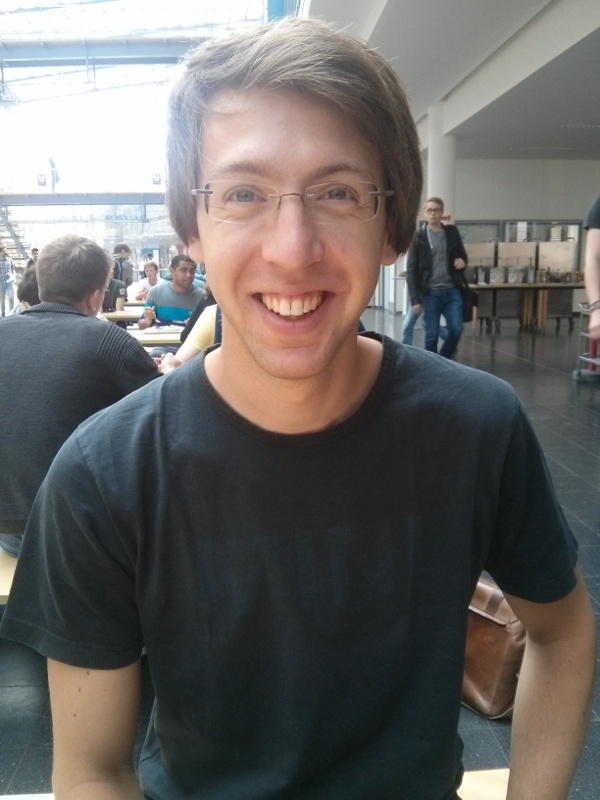
\includegraphics[height=3.4cm]{images/img_bjoern_small.jpg}&
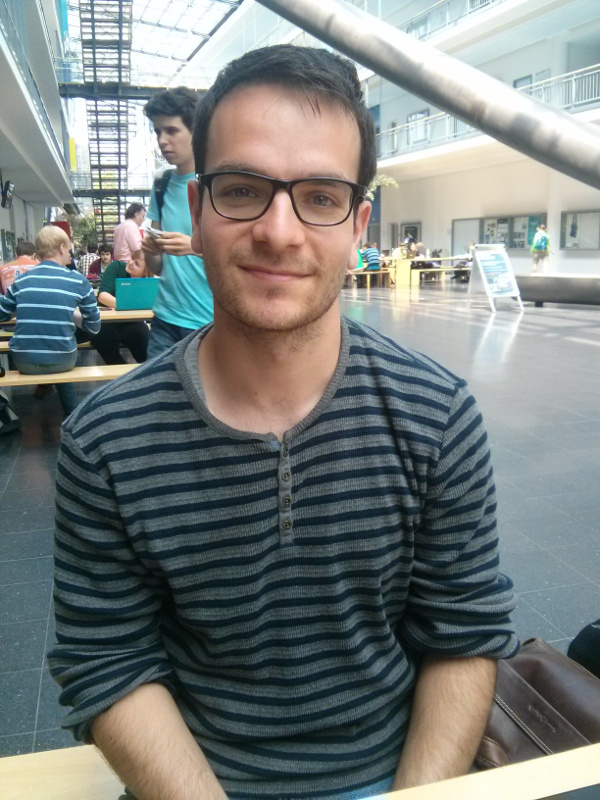
\includegraphics[height=3.4cm]{images/img_sebastian_small.jpg}&
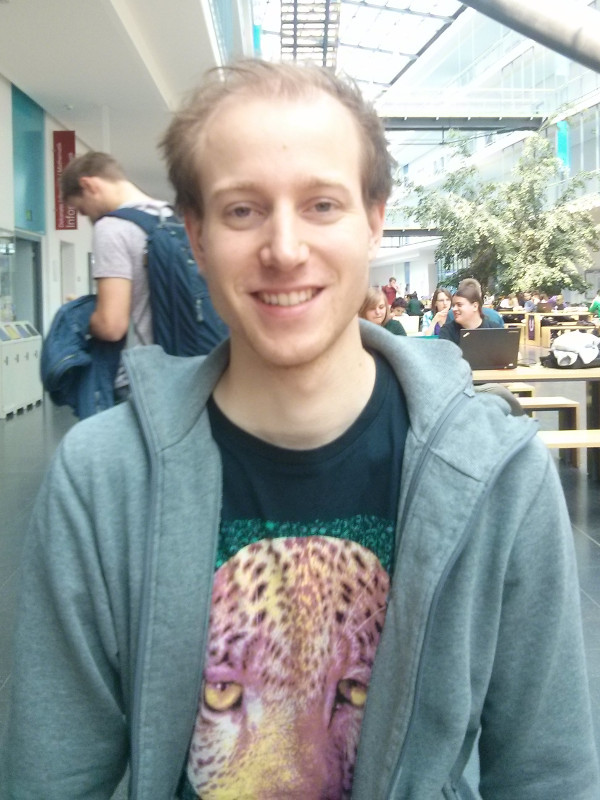
\includegraphics[height=3.4cm]{images/img_stefan_small.jpg}\\
Bj\"{o}rn Kirschner & Sebastian Schleemilch & Stefan Smarzly
\end{tabular}
\end{bigcenter}

\bigskip
\bigskip

\hrule
\bigskip
\bigskip


\bigskip

\textbf{Abstract:} blabla ... \todo{TODO!!!}

\newpage
\bigskip
\tableofcontents

\bigskip
\bigskip
\bigskip
\hrule

\bigskip
\bigskip

%\newpage

\section{Introduction}

This paper presents the final of \app, a solution to control access to university buildings via a mobile device communicating with a receiver at the door.
This communication works via near field communication (NFC).
Main contribution of the presented project is an Android application embedded in a holistic system which provides simple door access capabilities.
%Given the limited scope of the project, we start with a prototypical setup while striving for the system to eventually be employed by the TU München (TUM).

%Apart from this application we plan a prototypical implementation of a NFC reader using 



\subsubsection*{Problem description}

%\todo{ganzes Kap kürzen!}

Full-time students at TU München often face the problem that courses or seminars take place on a Saturday or a Sunday.
Since buildings at the university campus are generally closed at weekends, students have to ring for the security personnel to open the door.
But due to the number of students entering and leaving university buildings, door wardens hardly ever check the legitimacy of any entrant's business, i.e.~if they really are students.
This situation is unsatisfactory for all participants:

\begin{itemize}
\item Students needlessly have to wait for someone to open the door.
\item Door wardens get distracted from more important work.
\item Door wardens and university authorities cannot guarantee that entering people are students (or authorised persons in general).
\end{itemize}

\subsubsection*{Solution}

In order to overcome afore-mentioned problems, this paper presents a solution which allows students to authenticate at a door system and are granted or denied access automatically. This approach helps to...

\begin{itemize}
\item reduce possible waiting times for students,
\item unburden door wardens,
\item and guarantee that only students and other authorised persons are granted access.
\end{itemize}

A few areas in TUM buildings already use an access mechanism via the student card.
But for security reasons this student card solution is not ideal.
Because the card only identifies via an imprinted unique ID, reading and duplicating the card is possible.
For this reason we developed a smartphone solution which implements state of the art security mechanisms.
This solution has the potential to not only be used for main door entrances to the university but also to control access to chairs or other restricted areas.
It is an overall solution, relying solely on the user's smartphone.
 
 \subsubsection*{Structure of this paper}

The following chapter motivates the need for such a door access solution and sketches the project idea. Chapter \ref{sec:arch} then details the proposed technical architecture. Due to a several possible approaches, chapter \ref{sec:alt} justifies our design decisions. Finally, chapter \ref{sec:team} introduces all team members and chapter \ref{sec:plan} outlines a project plan.\todo{Anpassen} 

\section{Project Idea}



\subsection{Problem description}

Full-time students at TU München often face the problem that courses or seminars take place on a Saturday or a Sunday.
Since buildings at the university campus are generally closed at weekends, students have to ring for the security personnel to open the door. But due to the number of students entering and leaving university buildings, door wardens hardly ever check the legitimacy of any entrant's business, i.e.~if they really are students.\\
This situation is unsatisfactory for all participants:

\begin{itemize}
\item Students needlessly have to wait for someone to open the door.
\item Door wardens get distracted from more important work.
\item Door wardens and university authorities cannot guarantee that entering people are students (or authorised persons in general).
\end{itemize}

\subsection{Solution}

In order to overcome all problems mentioned in the previous chapter, we suggest that students authenticate at a door system and are granted or denied access automatically. This would...

\begin{itemize}
\item reduce possible waiting times for students,
\item unburden door wardens,
\item and guarantee that only students and other authorised persons are granted access.
\end{itemize}

Right now, in TUM there are existing some simple card readers for the Studentcard to access a few areas. For security reasons, the Studentcard solution is not ideal. The Studentcard access could be faked easily, since it has only an imprinted unique ID that could be read and printed easily to any other new Card. So a better solution would be the use of a smartphone where you can implement recent security mechanisms to control the access. This solution could not only be used for main door entrances to the university but also to control the access to the particular chairs. It would be an overall solution, with a smartphone as the prerequisite of course.

\section{Architectural Overview}
At the beginning, we thought about a robot (see figure \ref{img:robot1}) with two wheels (controlled by the two motors) in the front and a castor wheel in the back. The NUC and the Arduino sandwich are then put at the first level, at the barycenter of the wheels. The camera is placed at the top (second level).

\subsection{Registration with Backend}

\subsection{Authentication between Smartphone and NFC Reader}
\section{Design Alternatives}\label{sec:alt}
In the previous section, the overall architecture is presented without going into detail about the used hardware or how secure channels are implemented.
This section demonstrates some drafts for the concrete design of central parts of our project. 

\subsection{Hardware Setup}
A major part is a reliable communication link between an Android smartphone and a NFC reader.
To reach this goal, the NFC reader must support common NFC standards and stable transmission properties.
Therefore, we examine two different approaches to finally get a proper solution:
\begin{itemize}
	\item Raspberry Pi with the Explore-NFC reader cape by NXP \footnote{\url{http://www.nxp.com/demoboard/PNEV512R.html}}.
	\item Another smartphone with NFC capabilities and Android 4.4 or newer.
\end{itemize}

Raspberry Pi and Explore-NFC reader by NXP.
\begin{itemize}
	\item Advantage
	\begin{itemize}
		\item Cheap hardware.
		\item Available GPIOs for opening the door.
	\end{itemize}
	%apt
	\item Drawback
	\begin{itemize}
		\item SDK for interfacing with NFC cape might be unstable.
		\item No integrated Wifi and Bluetooth.
	\end{itemize}
\end{itemize}

Another Android smartphone with NFC support.
--> advantages / difficulties

\subsection{Protocols for Authentication between Smartphone and NFC Reader}

\subsubsection{Public-key Cryptography}

\subsubsection{Extended Randomized Hash Lock}

\section{Project Team}\label{sec:team}

\subsection{Name}
At the beginning, we thought about a robot (see figure \ref{img:robot1}) with two wheels (controlled by the two motors) in the front and a castor wheel in the back. The NUC and the Arduino sandwich are then put at the first level, at the barycenter of the wheels. The camera is placed at the top (second level).
\section{Action Planning and Scheduling}

At the beginning, we thought about a robot (see figure \ref{img:robot1}) with two wheels (controlled by the two motors) in the front and a castor wheel in the back. The NUC and the Arduino sandwich are then put at the first level, at the barycenter of the wheels. The camera is placed at the top (second level).

\end{document}